\section{Tuning}\label{sec:tuning}
In machine learning there is no default set of parameters or rule set which will
gaurantee optimal performance.
The only conclusive method to find optimal parameter values is to evaluate
each by comparison.
This can quickly lead to overfitting if the results are misinterpreted or
incorrectly measured.

The primary cause of overfitting is tuning on the entire dataset.
To reduce the chance of this, datasets should be split into development
and evaluation sets, on top of cross validation.
Although we don't do this here, we do use 10-times 10-fold cross validation as
described in Section~\ref{sec:acc_eval}.

The OOB error rate gives us an estimate of real-world performance, and we may
gain some insight into whether or not we are actaully gaining performance in
other metrics or overfitting by comparing this with the OOB error.


\subsection{Gridsearch}
The most basic form of parameter search is gridsearch.
A set of influential parameters are chosen, as well as a range of discrete
values to test.
Gridsearch then involves the exhaustive enumeration of all possible parameter
value combinations.

We test each combination using the usual evaluation mechanism with the following
search space:
\begin{itemize}
  \item Number of Estimators: 10, 100, 500, 5000, 10000
  \item Max features: $sqrt$, $log2$, $0.33*n$
\end{itemize}

The effect of each parameter is described in Section~\ref{sec:param}.
We have not tested other parameters due to the time cost of doing so.


\subsubsection{Results}

\begin{figure}[!htb]
  \centering
  \begin{subfigure}[b]{0.70\textwidth}
    \centering
    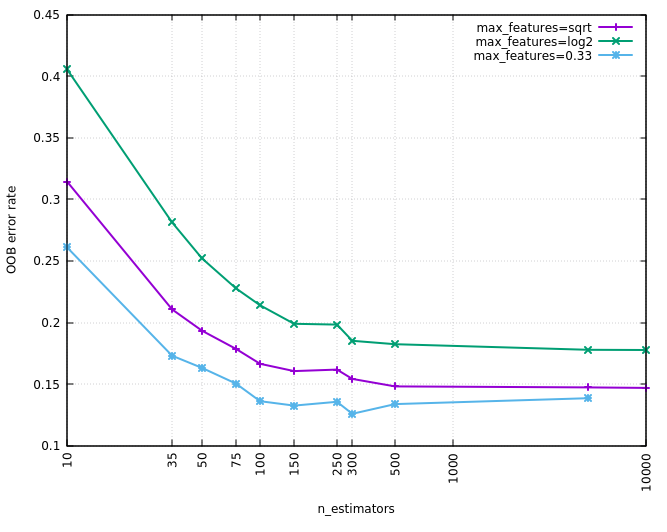
\includegraphics[width=1.0\textwidth]{plt_oob}
    \caption{OOB error}
    \label{fig:tuning_oob}
  \end{subfigure}\\
  \begin{subfigure}[b]{0.5\textwidth}
    \centering
    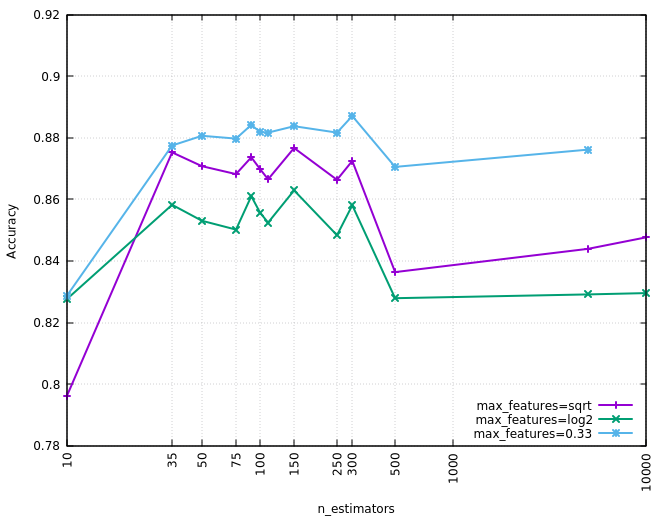
\includegraphics[width=1.0\textwidth]{plt_acc}
    \caption{Accuracy}
    \label{fig:tuning_acc}
  \end{subfigure}%
  \begin{subfigure}[b]{0.5\textwidth}
    \centering
    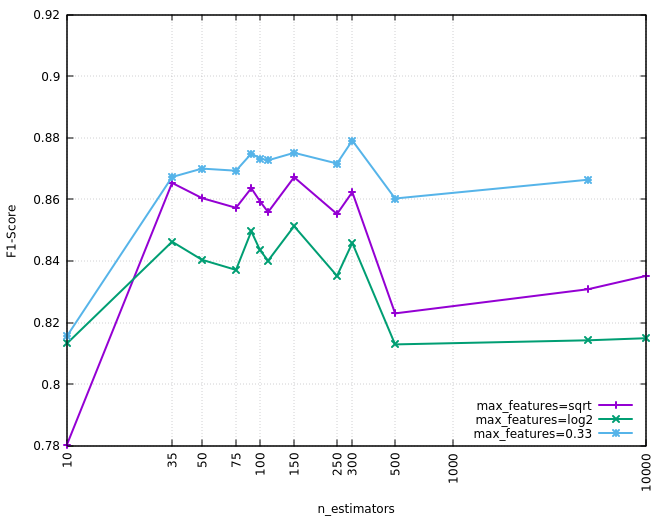
\includegraphics[width=1.0\textwidth]{plt_f1}
    \caption{F1-Score}
    \label{fig:tuning_f1}
  \end{subfigure}
%  \begin{subfigure}[b]{0.5\textwidth}
%    \centering
%    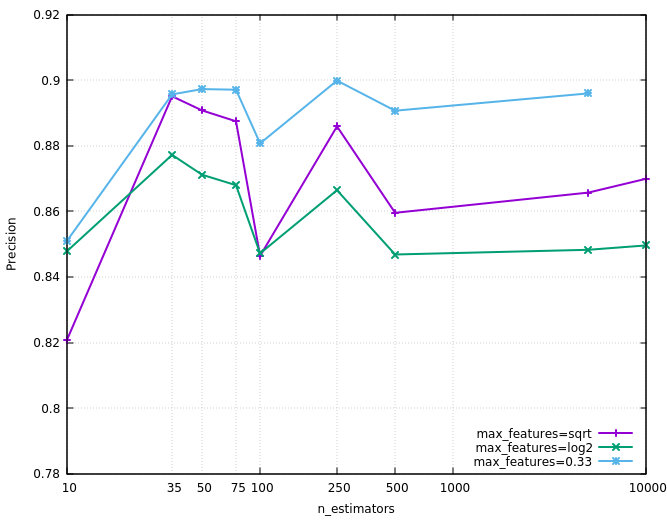
\includegraphics[width=1.0\textwidth]{plt_prc}
%    \caption{Precision}
%  \end{subfigure}%
%  \begin{subfigure}[b]{0.5\textwidth}
%    \centering
%    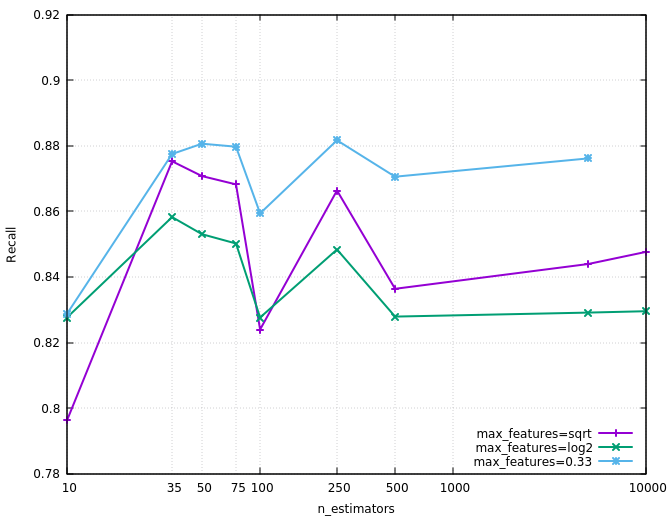
\includegraphics[width=1.0\textwidth]{plt_rec}
%    \caption{Recall}
%  \end{subfigure}
  \caption{Metrics over n. estimators for each max feature function}
  \label{fig:tuning}
\end{figure}

The OOB error rate (Figure~\ref{fig:tuning_oob}) shows that the random forest is
predicted to achieve peak
performance with $0.33 * n. features$ at around 300 estimators, rising outside
the stable range of $]150,500[$.
The error rate plateaus at about 500 estimators with other max feature functions.

Accuracy (Figure~\ref{fig:tuning_acc}) and F1-score (Figure~\ref{fig:tuning_f1})
show that peak performance is achieved between $]35,50[$
and $[150,500[$ estimators for all max feature functions.
Because the OOB error begins to stabalise at 100, it is likely that the latter
range is more indicative of real-world performance over the former.
The $0.33$ function specifically achieves the peak performance at 300 estimators.
This correlates with the OOB error curve.

The rise in accuracy at from 500 estimators is most likely attributed to
overfitting, especially as we consider the tendant rise in OOB error from that
point.
Performance improvements are generally observed with the increase in max features.
The linear max features function shows a smoother response and better
performance overall.\\

Without a completely independent validation data set it is impossible to perform
a truly representative evaluation.


\subsection{validation curves}
we tune based on best performing params in gsearch
possibly biased towards validation dataset
for better generalization estimation compute score on different set
(already mentioned above)

we can use this to check over/under fitting?
check influence of single parameter on training and validation scores
if both are low, clf is undefitting
if training is high, valid is low, clf is overfitting
low training, high validation not possible usually

coarse-to-fine search gridsearch, if we have the time

\subsection{Learning Rate}
learning curve
shows validation/training score for varying train sample count.
shows how clf may benefit from additional samples if at all
shows if clf suffers from variance or bias error
if validation and training score converge to a low value with more training samples,
we don't benefit. might have to change parameters or choose different clf which
has lower bias

if training score is higher than valid score, we benefit from adding training
samples probably, increasing generalisation

is this useful for RF?
